\section{Conception}
    Dans le but de limiter l'utilisation de la mémoire et de réduire le temps d'entraînement, les réseaux de neurones n'utilisent pas les images Full HD (1920x1080) à l'entrée, mais plutôt des images redimensionnées par un facteur de 4. Les images d'entrée des réseaux de neurones ont une résolution de 480x270. La sortie de tous les réseaux de neurones correspond à une matrice d'erreur de 16x9 éléments parce que les images sont divisées en 144 régions comme décrit à la section \ref{sec:definition_projet}. Les régions ont une résolution 30x30 pour les images d'entrée des réseaux de neurones (120x120 pour les images Full HD). Pour l'ensemble des réseaux de neurones développés, le champ récepteur des neurones de sortie est de 60x60 (240x240 pour les images Full HD) parce que nous avons émis l'hypothèse que le voisinage de chaque région a une influence sur la région correspondant au neurone de sortie. Chaque élément de la matrice d'erreur de 16x9 correspond à l'erreur quadratique de reconstruction de la région de l'image d'entrée correspondante.\\
    
    Plusieurs réseaux de neurones ont été conçus pour déterminer le meilleur type de réseau à utiliser dans ce contexte. Certains sont des auto-encodeurs travaillant sur les pixels directement et d'autres ont un réseau de neurones pour l'extraction de caractéristiques, suivi d'un auto-encodeur travaillant sur les caractéristiques extraites. 

\subsection{Choix des métriques}
    L'entraînement se fait de façon non supervisée, donc il  a été décidé d'utiliser la fonction de coût d'entraînement du réseau définie par l'équation suivante. À l'aide de celle-ci, les réseaux de neurones apprennent à reconstruire les régions des images d'entraînement.
    
    \begin{equation}
        L = \sum_{i,j} \mathbf{S}_{i,j} \text{, où } \mathbf{S} \text{ est la matrice de sortie du réseau de neurone}
    \end{equation}
    
    Pour mesurer les performances des réseaux de neurones sur les données de validation et de test, l'utilisation des courbes ROC a été choisi puisque notre problème équivaut à un problème de classification deux classes où la classe est déterminée à l'aide d'un seuil. La courbe ROC est une bonne métrique dans ce cas. Pour permettre la comparaison des réseaux de neurones avec différents hyperparamètres et établir le meilleur type de réseau de neurones pour la situation, l'aire sous la courbe ROC a été utilisée. Plus l'aire sous la courbe est grande, plus que le réseau est bon. Pour calculer la courbe ROC, le nombre de vrais positifs et de faux positifs a été calculé pour différentes valeurs de seuil.

\subsection{Architecture des modèles}
    La figure \ref{fig:architecture_bloc_dense} présente l'architecture d'un bloc dense utilisé dans certains réseaux de neurones. Ce bloc peut être configuré à l'aide de \(N_C\) et de \(t\). 
    \begin{figure}[H]
        \centering
        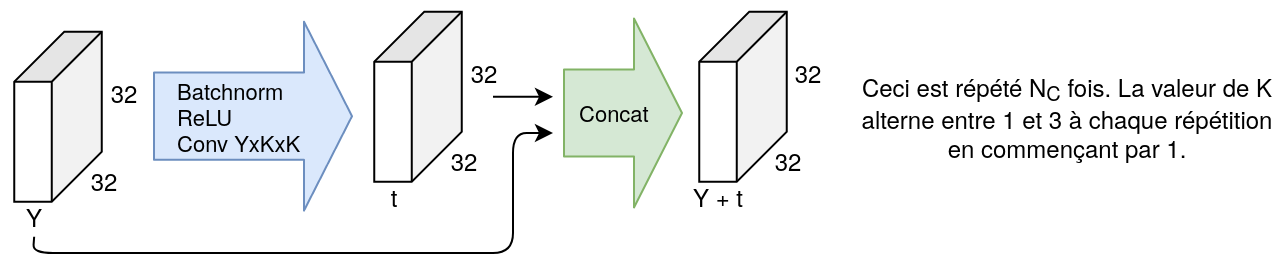
\includegraphics[width=12cm]{images/Architecture_DenseBlock.png}
        \caption{Architecture d'un bloc dense}
        \label{fig:architecture_bloc_dense}
    \end{figure}

    Certains réseaux de neurones font l'extraction de caractéristiques pour ensuite les utiliser dans un auto-encodeur. Tous ces réseaux utilisent le même auto-encodeur. Son architecture est présentée à la figure  \ref{fig:architecture_autoencoder_caracteristique}. L'entrée possède un nombre variable de canaux en entrée et a la même taille que la matrice d'erreurs. Ceci est dans le but que chaque vecteur de dimensions \(N_C\)x1x1 du tenseur d'entrée de dimensions \(N_C\)x16x9 correspond aux caractéristiques de chaque région de l'image. Les couches de ce réseau de neurones sont composées de convolutions 1x1 et de ReLU. Le nombre de canaux diminue à chaque couche dans l'encodeur et augmente dans le décodeur. Par conséquent, l'auto-encodeur apprend à réduire la dimensionnalité des caractéristiques de chaque région de l'image. La sortie de l'auto-encodeur correspond à l'erreur de reconstruction des caractéristiques des régions.
    \begin{figure}[H]
        \centering
        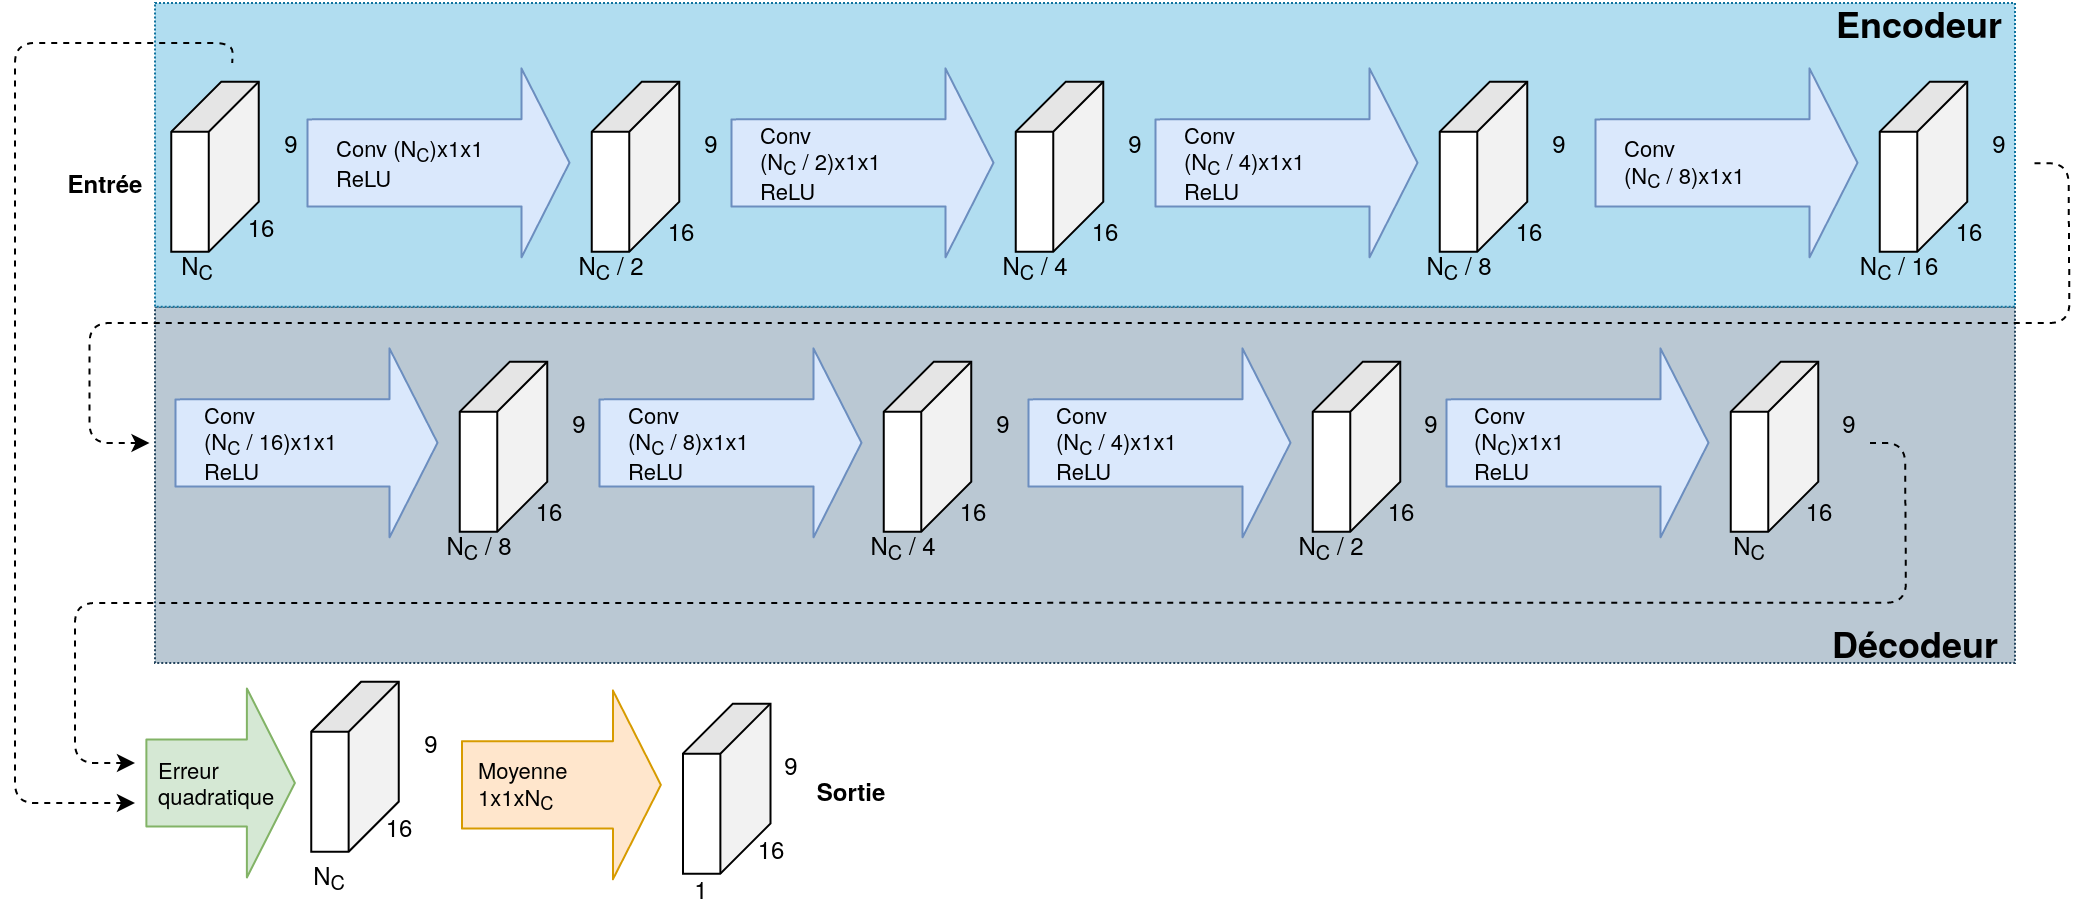
\includegraphics[width=17cm]{images/Architecture_FeatureAutoencoder.png}
        \caption{Architecture de l'auto-encodeur des caractéristiques}
        \label{fig:architecture_autoencoder_caracteristique}
    \end{figure}

\subsubsection{Auto-encodeur à base de couche convolutive appliqué sur l'image}
    Un réseau de neurones de type auto-encodeur reconstruisant l'image en entrée à été conçu. L'architecture de ce réseau est présentée à la figure \ref{fig:architecture_cnn_autoencoder}. Le réseau est configurable à l'aide de \(N_A\) et de \(N_B\). \(N_A\) permet de choisir le nombre de canaux après la première convolution de l'encodeur, tandis que \(N_B\) permet de choisir le taux de grossissement du nombre de canaux après chaque convolution de l'encodeur. Le décodeur est symétrique par rapport à l'encodeur. À la sortie du décodeur, il y a une interpolation bilinéaire, car il n'était pas possible de respecter en même temps le champ récepteur et le fait que l'image en entrée et celle en sortie aient la même taille parce que certains \textit{MaxPool} ne donnent pas une sortie de type \textit{same}. Alors, la solution la plus simple était d'utiliser une interpolation bilinéaire. La dernière fonction d'activation du décodeur est la fonction sigmoïde parce que les valeurs des pixels d'une image sont entre 0 et 1. La sortie du réseau de neurones est l'erreur quadratique moyenne de la reconstruction de chaque région. Ce réseau de neurones sera appelé modèle A dans la suite du document.
    \begin{figure}[H]
        \centering
        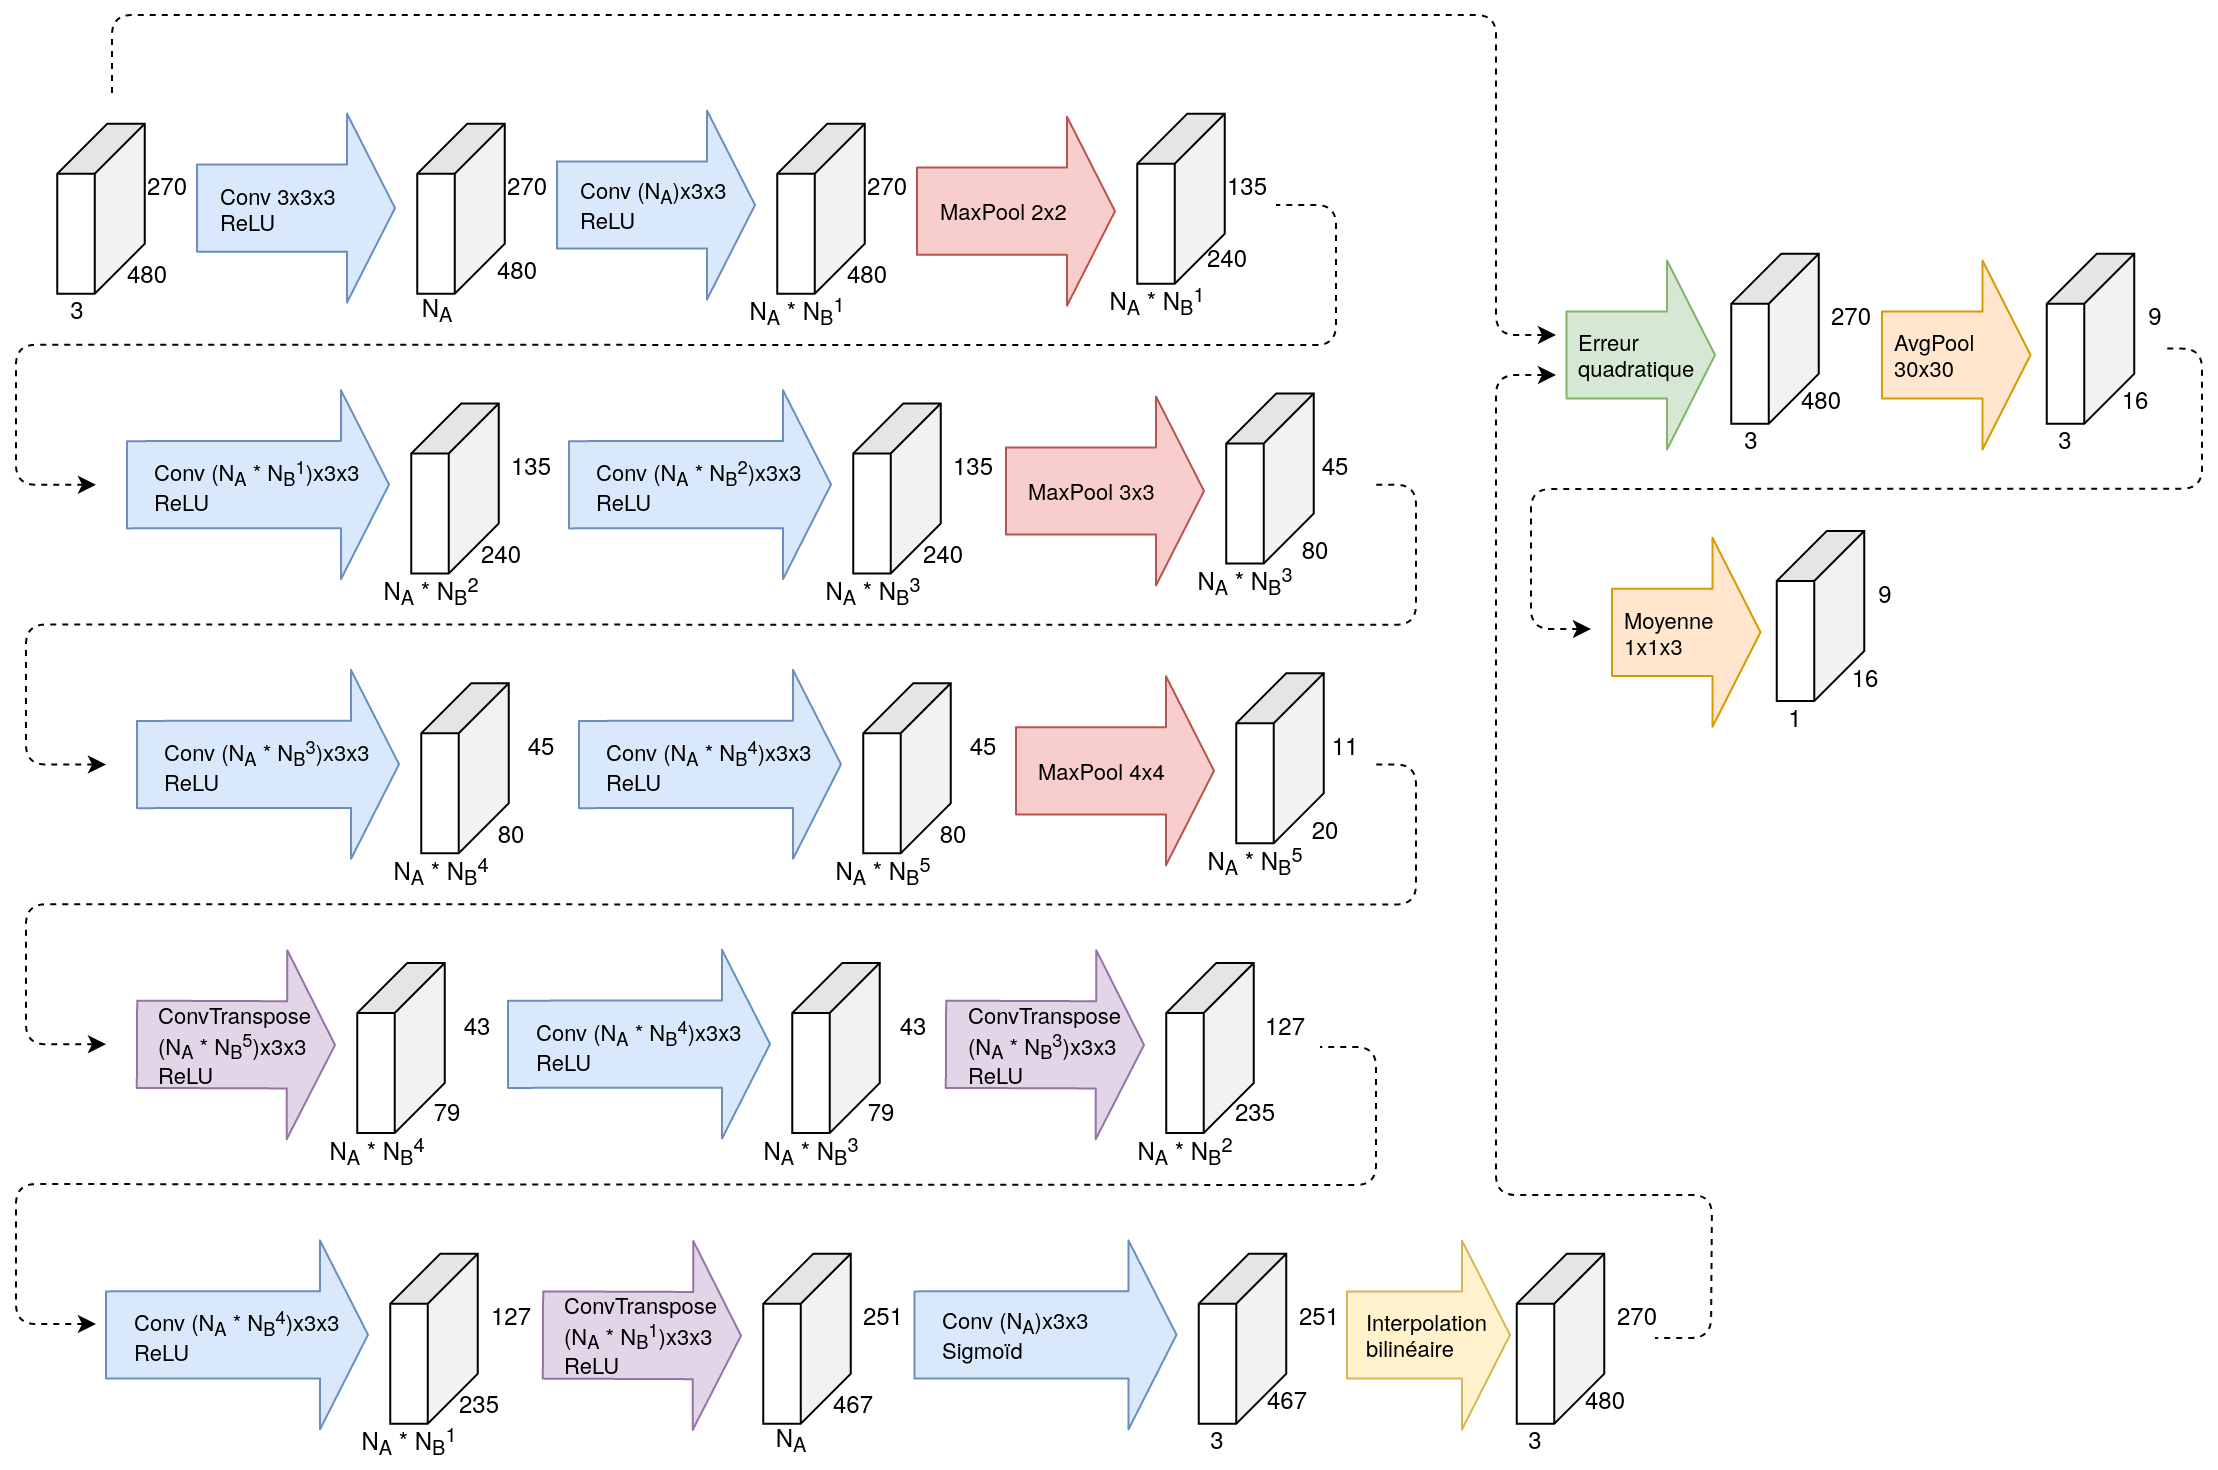
\includegraphics[width=17cm]{images/Architecture_CnnAutoencoder.png}
        \caption{Architecture de l'auto-encodeur à base de couche convolutive appliqué sur l'image}
        \label{fig:architecture_cnn_autoencoder}
    \end{figure}

\subsubsection{Auto-encodeur variationnel à base de couche convolutive appliqué sur l'image}
    Il a été décidé de développer un auto-encodeur variationnel dans le but de vérifier si le fait de contraindre la sortie de l'encodeur permet d'améliorer les performances. Par conséquent, l'architecture de l'auto-encodeur variationnel présenté à la figure \ref{fig:architecture_cnn_vae} est très semblable à celle du modèle A. Les seules différences concernent la sortie de l'encodeur et l'entrée du décodeur. La sortie de l'encodeur correspond à une distribution de probabilité normale multidimensionnelle où la matrice de covariance est une diagonale. L'entrée du décodeur est un point échantillonné la cette distribution de probabilité. Ce réseau de neurones sera appelé modèle B dans la suite du document.
    \begin{figure}[H]
        \centering
        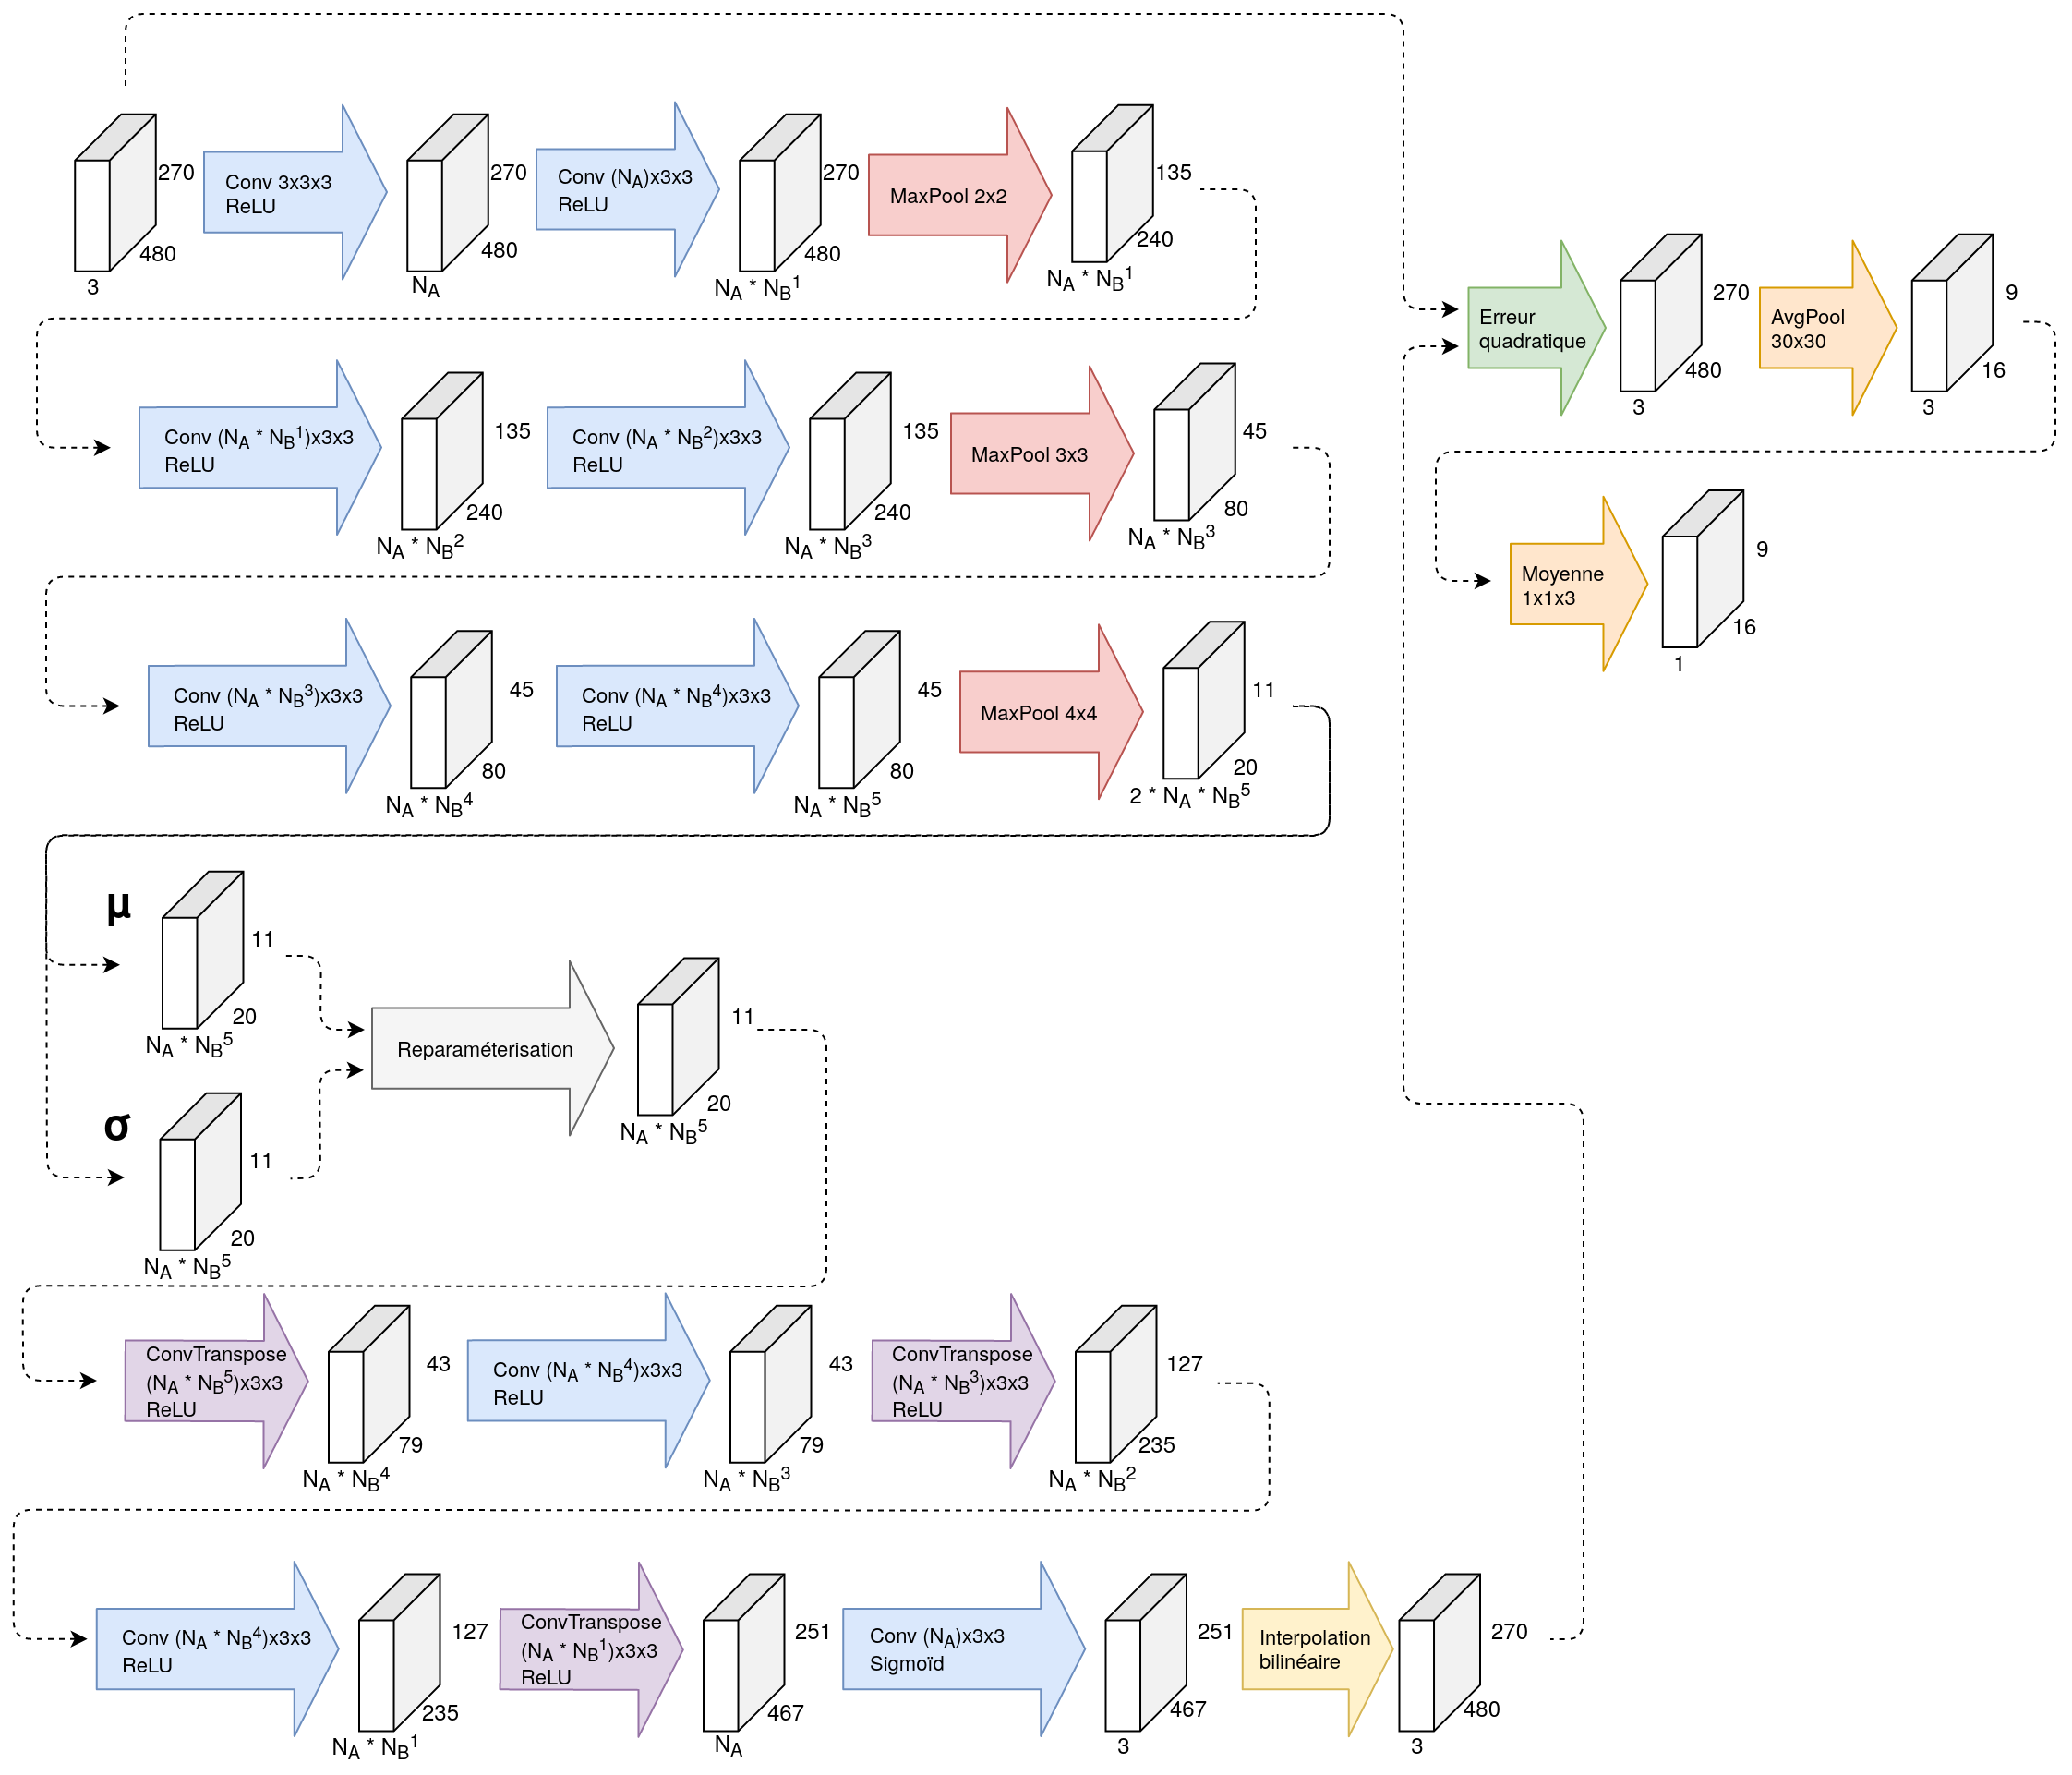
\includegraphics[width=17cm]{images/Architecture_CnnVae.png}
        \caption{Architecture de l'auto-encodeur variationnel à base de couche convolutive appliqué sur l'image}
        \label{fig:architecture_cnn_vae}
    \end{figure}

\subsubsection{Réseau de neurones convolutif extrayant des caractéristiques}
    La sortie du réseau de neurones convolutif présenté à la figure \ref{fig:architecture_small_cnn} est envoyée à l'entrée de l'auto-encodeur des caractéristiques (figure \ref{fig:architecture_autoencoder_caracteristique}) pour que la sortie de l'auto-encodeur des caractéristiques soit les erreurs de reconstruction des régions. Le réseau de neurones convolutif sert extraire des caractéristiques de chaque région de l'image. Le réseau est configurable à l'aide de \(N_A\) et de \(N_B\). Les effets de ces paramètres sont les mêmes que dans le modèle A. À la sortie du réseau de neurones convolutif, il y a l'application d'une \textit{BatchNorm} dans le but de limiter la plage dynamique des caractéristiques de chaque région et d'une interpolation bilinéaire pour obtenir la bonne taille. L'interpolation bilinéaire est nécessaire pour les mêmes raisons que le modèle A. La combinaison de ces deux réseaux de neurones sera appelée modèle C dans la suite du document.
    \begin{figure}[H]
        \centering
        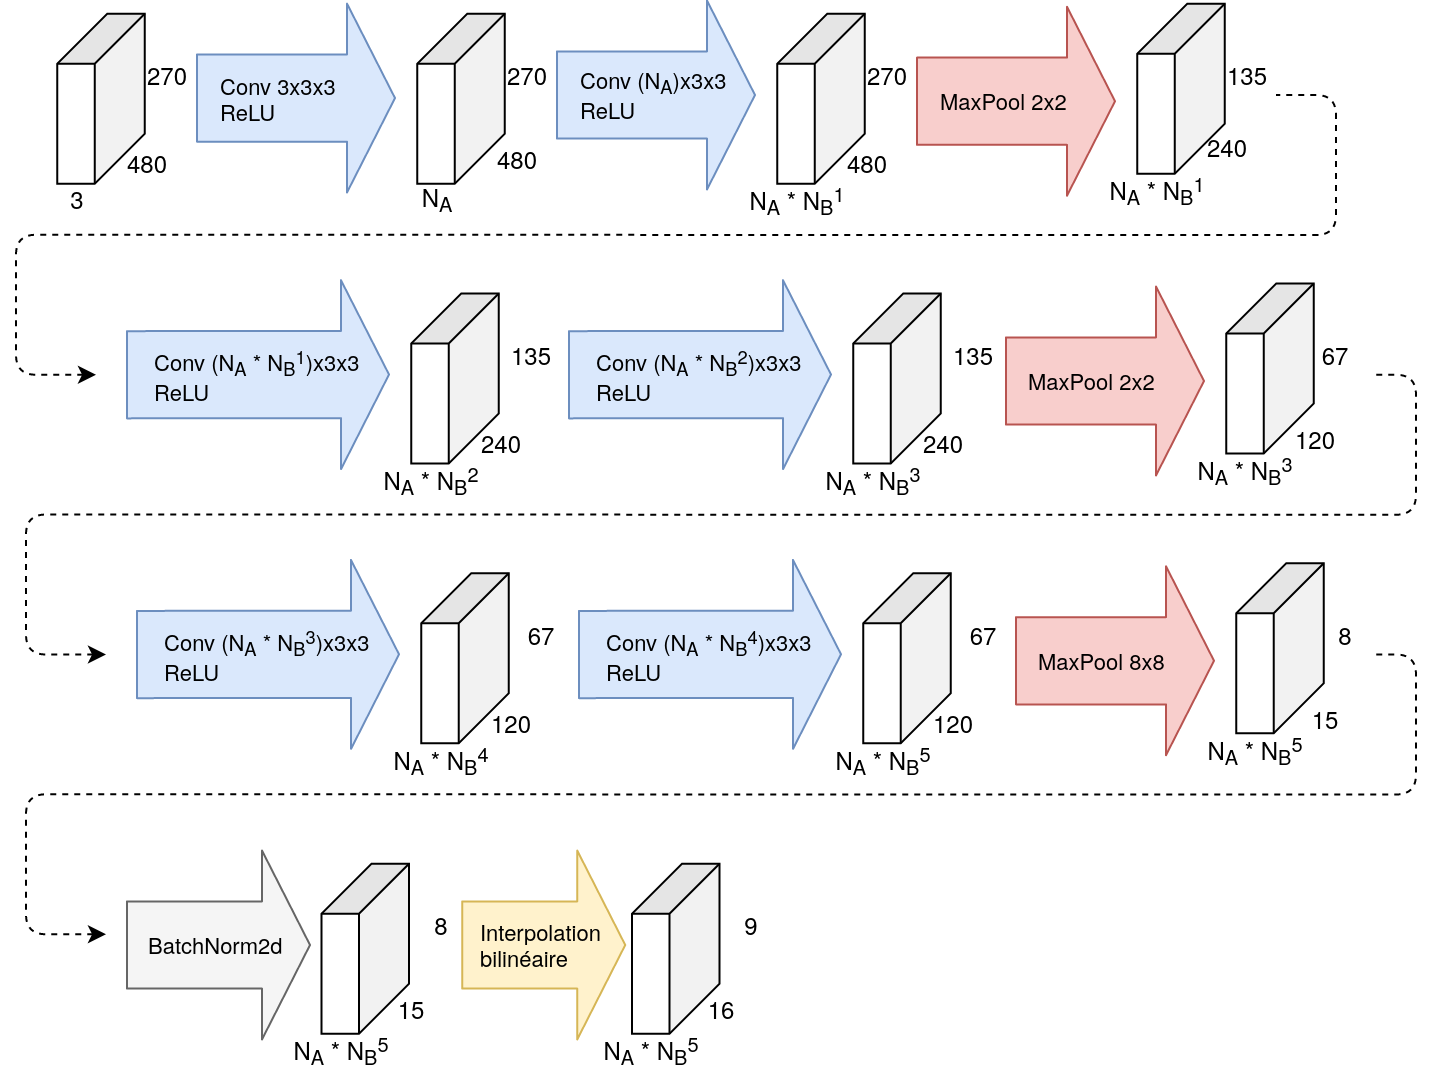
\includegraphics[width=17cm]{images/Architecture_SmallCnnWithAutoencoder.png}
        \caption{Architecture du réseau de neurones convolutif extrayant des caractéristiques}
        \label{fig:architecture_small_cnn}
    \end{figure}

\subsubsection{Réseau de neurones à base de blocs denses extrayant des caractéristiques}
    \begin{figure}[H]
        \centering
        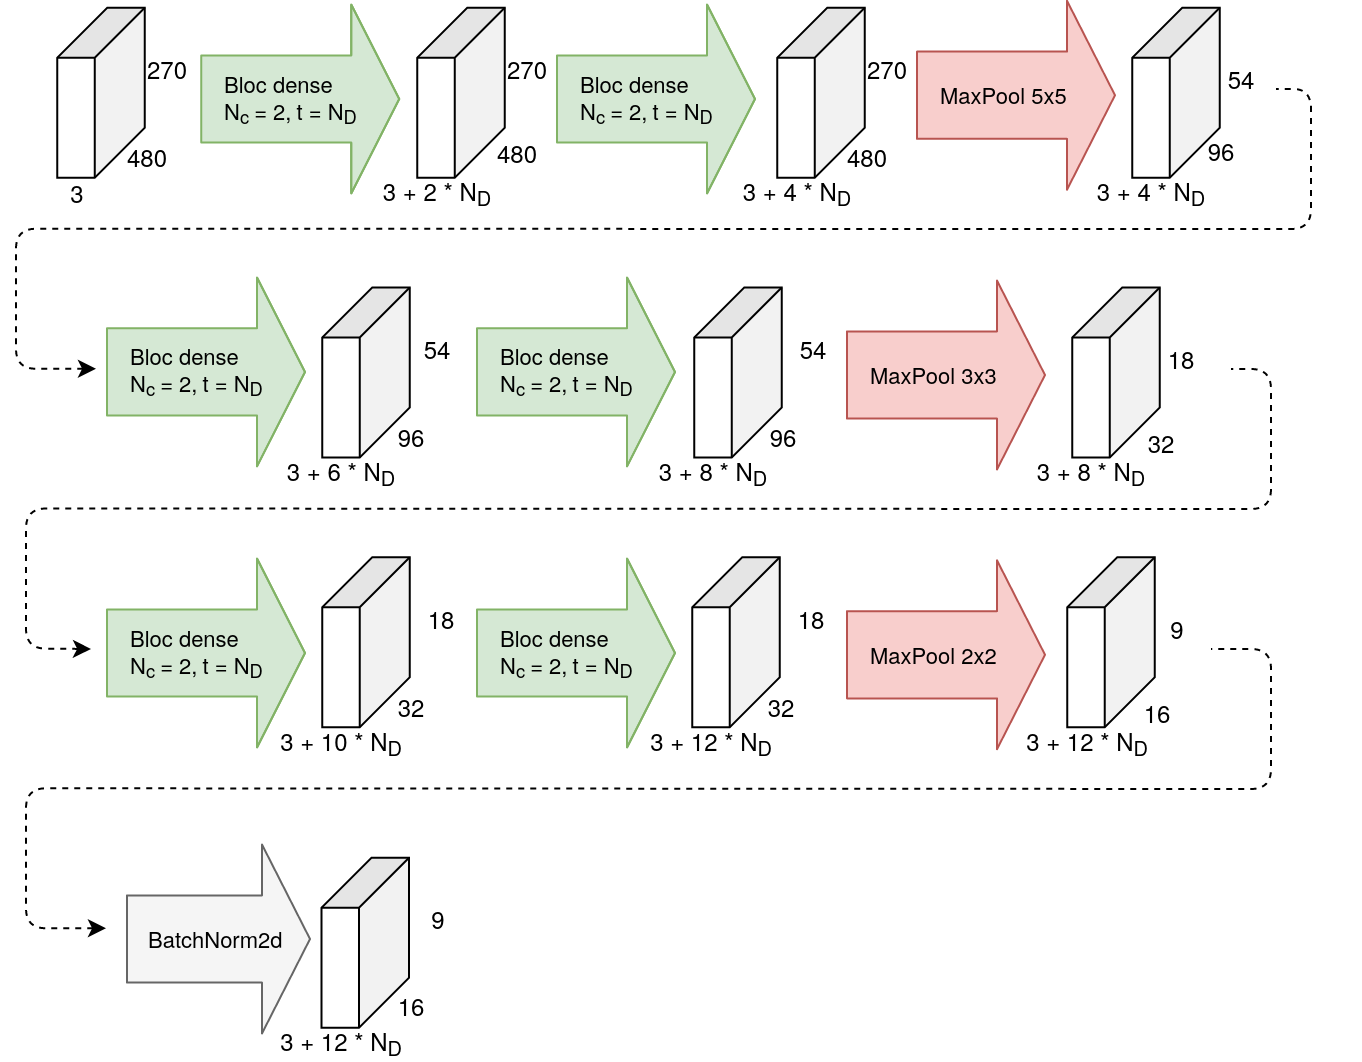
\includegraphics[width=17cm]{images/Architecture_SmallCnnWithAutoencoderDenseBlocks.png}
        \caption{Architecture du réseau de neurones à base de blocs denses extrayant des caractéristiques}
        \label{fig:architecture_small_cnn_dense_bloc}
    \end{figure}

\subsection{Réseau de neurones utilisant un \textit{backend} VGG16 pour l'extraction des caractéristiques}
    La sortie du réseau de neurones utilisant un \textit{backend} VGG16 présenté à la figure \ref{fig:architecture_vgg16} est envoyée à l'entrée de l'auto-encodeur des caractéristiques (figure \ref{fig:architecture_autoencoder_caracteristique}) pour que la sortie de l'auto-encodeur des caractéristiques soit les erreurs de reconstruction des régions. Les 8 premières couches de VGG16, suivi d'un \textit{MaxPool} 8x8 a été utilisé pour obtenir le bon champ récepteur. Il y a l'utilisation d'une \textit{BatchNorm} et d'une interpolation bilinéaire pour les mêmes raisons que le modèle C. La combinaison de ces deux réseaux de neurones sera appelée modèle E dans la suite du document.
    \begin{figure}[H]
        \centering
        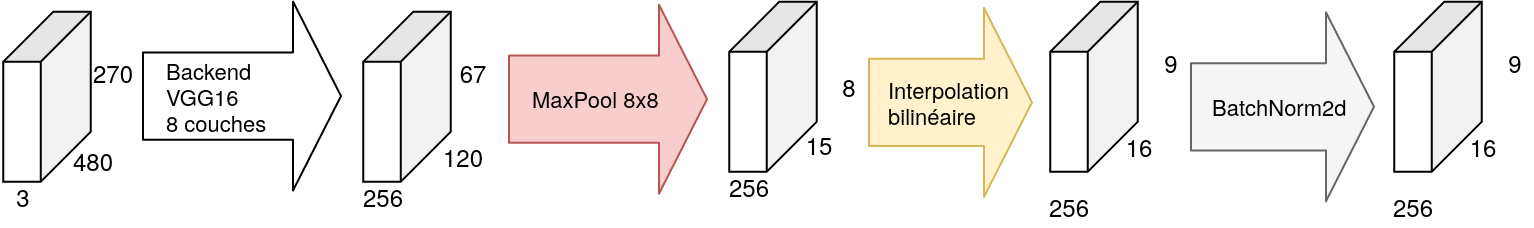
\includegraphics[width=12cm]{images/Architecture_Vgg16BackendAutoencoder.png}
        \caption{Architecture du réseau de neurones utilisant un \textit{backend} VGG16 pour l'extraction des caractéristiques}
        \label{fig:architecture_vgg16}
    \end{figure}

\subsection{Augmentation des données}
    